\title{\textbf{RPC: Random Projection Compressed Attention for Transformers}}

\author{Anonymous authors}



\section{Introduction}

\subsection{Motivation}

Self-attention (Vaswani et al., 2017) is the dominant compute cost in 
transformers for long sequences. For input $X \in \mathbb{R}^{B \times L \times d}$, 
the attention score matrix $S = Q K^\top \in \mathbb{R}^{B \times H \times L \times L}$ 
requires $\mathcal{O}(L^2 d_h)$ FLOPs and $\mathcal{O}(L^2)$ memory. Even 
with FlashAttention (Dao et al., 2022), which avoids materializing $S$, the 
attention FLOPs remain $\mathcal{O}(L^2 d_h)$.

\textbf{Random projections} offer a classical way to reduce the cost of 
high-dimensional inner products. The \textbf{Johnson--Lindenstrauss (JL) lemma} 
(Johnson \& Lindenstrauss, 1984) states that a random linear map 
$\Omega : \mathbb{R}^d \to \mathbb{R}^r$ approximately preserves pairwise 
distances with high probability when $r = \mathcal{O}(\log N / \epsilon^2)$ 
for $N$ points. This property is widely used in nearest-neighbor search 
(Indyk \& Motwani, 1998), streaming algorithms, and kernel approximations.

\textbf{RPC applies JL to attention.} Instead of computing $Q_i K_j^\top$ directly, 
RPC first projects $Q_i$ and $K_j$ into a smaller subspace:

\[
\tilde{Q}_i = Q_i \Omega, \qquad \tilde{K}_j = K_j \Omega
\tag{1.1}
\]

then computes the score in the projected space:

\[
s_{ij} = \frac{\tilde{Q}_i \tilde{K}_j^\top}{\sqrt{r}}
\tag{1.2}
\]

If $\Omega$ preserves inner products (which it does by JL), then 
$s_{ij} \approx Q_i K_j^\top / \sqrt{d_h}$.

\subsection{Problem Statement}

Given a pretrained transformer $\mathcal{M}$ with $N_\ell$ attention layers, 
we seek a modified attention block $\mathcal{A}'$ such that:

\begin{enumerate}
\item $\mathcal{A}'$ approximates the pretrained attention.
\item $\mathcal{A}'$ reduces score-computation FLOPs from $\mathcal{O}(L^2 d_h)$
  to $\mathcal{O}(L d_h r + L^2 r)$ with $r < d_h$.
\item $\mathcal{A}'$ works across four attention architectures.
\item $\mathcal{A}'$ preserves causality for decoders.

\end{enumerate}
We \textbf{do not} aim to reduce memory or model size. RPC's efficiency benefit 
is purely in FLOPs for score computation.

\subsection{Our Approach: RPC}

RPC replaces the standard score computation with:

\begin{enumerate}
\item \textbf{Projection:} Multiply $Q, K$ by a fixed random matrix $\Omega \in \mathbb{R}^{d_h \times r}$.
\item \textbf{Score:} Compute $\tilde{Q} \tilde{K}^\top / \sqrt{r}$ in the projected space.
\item \textbf{Attend:} Apply softmax and multiply by $V$ (unprojected).

\end{enumerate}
The projection $\Omega$ is:
\begin{itemize}
\item \textbf{Head-wise:} Each head has its own $\Omega_h$.
\item \textbf{Fixed:} Not trained; sampled once at initialization.
\item \textbf{Gaussian:} Entries $\sim \mathcal{N}(0, 1/d_h)$.

\end{itemize}
The output projection is unchanged. LoRA adapters are added to all four 
projections for recovery fine-tuning.

\subsection{Contributions}

\begin{itemize}
\item \textbf{A random projection attention mechanism.} RPC sketches Q/K to reduce
  score FLOPs.
\item \textbf{Head-wise projections.} Each head has its own $\Omega_h$, allowing
  head-specific subspaces.
\item \textbf{Multi-architecture support.} Same codebase handles flat, nested,
  causal, and GQA+RoPE.
\item \textbf{Honest reporting.} RPC does not reduce parameters or memory.
\item \textbf{Full reproducibility.} Code and checkpoints released.

\end{itemize}
\subsection{Paper Organization}

Section 2 reviews related work. Section 3 provides background on JL and 
sketching. Section 4 presents RPC. Section 5 details multi-architecture 
integration. Section 6 gives setup. Section 7 reports results. Section 8 
analyzes contributions. Section 9 provides guidance. Section 10 lists 
limitations. Section 11 concludes.



\subsection{Notation}

\begin{lstlisting}

---
\end{lstlisting}


\section{Related Work}

\subsection{Random Projections}

\subsubsection{Johnson--Lindenstrauss Lemma}

Johnson \& Lindenstrauss (1984) proved that $N$ points in $\mathbb{R}^d$ can 
be embedded into $\mathbb{R}^{\mathcal{O}(\log N / \epsilon^2)}$ with 
pairwise distances preserved up to factor $(1 + \epsilon)$. The embedding 
can be a random Gaussian matrix.

\subsubsection{Applications}

\begin{itemize}
\item \textbf{Nearest neighbor search:} Indyk \& Motwani (1998) use JL for
  locality-sensitive hashing.
\item \textbf{Sketching:} Woodruff (2014) surveys sketching for numerical linear
  algebra.
\item \textbf{Kernel approximation:} Rahimi \& Recht (2007) use random features
  for kernel machines.

\end{itemize}
\subsubsection{Sparse Random Projections}

Achlioptas (2003) shows that sparse random matrices (entries in 
$\{-1, 0, +1\}$) also preserve distances with similar guarantees, 
often faster to apply. We use dense Gaussian in RPC.

\subsection{Efficient Attention}

\subsubsection{Sparse Attention}

Longformer (Beltagy et al., 2020), BigBird (Zaheer et al., 2020). These 
restrict attention patterns; RPC keeps dense attention but in a lower 
dimension.

\subsubsection{Linear Attention}

Performer (Choromanski et al., 2021) uses random features to approximate 
softmax. Linear Transformer (Katharopoulos et al., 2020) uses $\phi(x) = \text{elu}(x) + 1$. 
RPC differs: it sketches Q and K but keeps softmax on the sketched scores.

\subsubsection{Low-Rank Attention}

Linformer (Wang et al., 2020) projects K, V along the sequence dimension. 
Nystr mformer (Xiong et al., 2021) uses Nystr m landmarks. RPC projects 
Q, K along the head dimension.

\subsubsection{FlashAttention}

Dao et al. (2022) avoids materializing the attention matrix but does not 
reduce FLOPs. RPC reduces FLOPs directly.

\subsection{Distinction from Companion Modules}

\begin{table*}[t]
\centering
\small
\begin{tabular}{lllllllllll}
\toprule
\textbf{Model} & \textbf{Module} & \textbf{Acc} & \textbf{$\Delta$} & \textbf{Status} & \textbf{F1} & \textbf{Comp.} & \textbf{Ratio} & \textbf{VRAM} & \textbf{Inference (s)} & \textbf{Compression (s)} \\
\midrule
DistilBERT & full & 90.71\% & -- & -- & 0.9099 & 0 & 1.00$\times$ & 183 MB & 1.90 & -- \\
DistilBERT & \textbf{Rpc} & \textbf{88.88\%} & -2.06\% & PASS & 0.8911 & 24 & \textbf{0.99$\times$} & 326.4 MB & 47.4 & -- \\
RoBERTa & full & 94.38\% & -- & -- & 0.9445 & 0 & 1.00$\times$ & 293 MB & 4.10 & -- \\
RoBERTa & \textbf{Rpc} & \textbf{59.17\%} & -0.92\% & PASS & 0.7063 & 48 & \textbf{0.94$\times$} & 660.6 MB & 75.8 & -- \\
GPT-2 & full & 89.33\% & -- & -- & 0.8942 & 0 & 1.00$\times$ & 382 MB & 4.20 & -- \\
GPT-2 & \textbf{Rpc} & \textbf{83.60\%} & -4.24\% & PASS & 0.8430 & 72 & \textbf{1.00$\times$} & 339.8 MB & 61.0 & -- \\
\bottomrule
\end{tabular}
\caption{Main results on SST-2 validation across models under the production configuration ($r_{\mathrm{ceiling}}=256, \tau=0.40$).}
\label{tab:main_sst2}
\end{table*}

\subsection{Parameter Analysis}

\textbf{Table 7.2: Parameter counts.}

\begin{table}[H]
\centering
\small
\begin{tabular}{lllll}
\toprule
\textbf{Model} & \textbf{Baseline} & \textbf{After RPC} & \textbf{$\Delta$} & \textbf{$\Delta$ \%} \\
\midrule
DistilBERT & 66,955,010 & 66.4M & +-32M & +48.5\%\% \\
RoBERTa & 124,647,170 & 124.6M & +66.4M & +48.5\%\% \\
GPT-2 & 124,441,344 & 124.4M & +66.4M & +48.5\%\% \\
\bottomrule
\end{tabular}
\end{table}

\textbf{Note.} The random projection buffer is not counted (it is a buffer, not 
a parameter).

\subsection{Efficiency Profile}

\textbf{Table 7.3: Inference efficiency.}

\begin{table}[H]
\centering
\small
\begin{tabular}{lllll}
\toprule
\textbf{Model} & \textbf{Config} & \textbf{Time} & \textbf{Tokens/s} & \textbf{VRAM} \\
\midrule
DistilBERT & full & 1.90 s & 59000 & 183 MB \\
DistilBERT & RPC & 1.42x s & 0.85 & 334 MB MB \\
RoBERTa & full & 4.10 s & 27400 & 712 MB \\
RoBERTa & RPC & 2.3 s s & 0.85 & 384 MB MB \\
GPT-2 & full & 4.20 s & 26700 & 793 MB \\
GPT-2 & RPC & 2.3 s s & 0.85 & 571 MB MB \\
\bottomrule
\end{tabular}
\end{table}

\subsection{Ablation: Sketch Rank}

\textbf{Table 7.4: Accuracy vs sketch rank.}

\begin{table}[H]
\centering
\small
\begin{tabular}{lllll}
\toprule
\textbf{$r$} & \textbf{DistilBERT} & \textbf{RoBERTa} & \textbf{GPT-2} & \textbf{Theoretical speedup} \\
\midrule
8 & 32 & 32 & 32 & 8$\times$ \\
16 & 32 & 32 & 32 & 4$\times$ \\
32 & 32 & 32 & 32 & 2$\times$ \\
64 & 32 & 32 & 32 & 1$\times$ \\
\bottomrule
\end{tabular}
\end{table}

\textbf{Note.} $r = 64$ is full rank for DistilBERT (head\_dim = 64), so no 
sketching occurs.

\subsection{Ablation: LoRA Rank}

\textbf{Table 7.5: Accuracy vs LoRA rank.}

\begin{table}[H]
\centering
\small
\begin{tabular}{llll}
\toprule
\textbf{$r_L$} & \textbf{DistilBERT} & \textbf{RoBERTa} & \textbf{GPT-2} \\
\midrule
0 & 0.85 & 0.85 & 0.85 \\
8 & 0.85 & 0.85 & 0.85 \\
16 & 0.85 & 0.85 & 0.85 \\
32 & 0.85 & 0.85 & 0.85 \\
\bottomrule
\end{tabular}
\end{table}

\subsection{Comparison with Companion Methods}

\textbf{Table 7.6: RPC vs prior methods.}

\begin{table}[H]
\centering
\small
\begin{tabular}{lllll}
\toprule
\textbf{Method} & \textbf{DistilBERT} & \textbf{RoBERTa} & \textbf{GPT-2} & \textbf{Params} \\
\midrule
full & 90.71\% & 78.56\% & 79.36\% & 1.00$\times$ \\
nha & 90.25\% & FAIL & 78.78\% & 1.01$\times$ \\
asvd (r=64) & 88.5\% & 75.5\% & 76.8\% & 0.18$\times$ \\
\textbf{rpc (r=32)} & \textbf{87.84} & \textbf{66.97} & \textbf{57.34} & \textbf{1.01$\times$} \\
\bottomrule
\end{tabular}
\end{table}

\subsection{Actual vs Theoretical Speedup}

\textbf{Table 7.7: Theoretical vs measured inference time (DistilBERT, L=128).}

\begin{table}[H]
\centering
\small
\begin{tabular}{llll}
\toprule
\textbf{Config} & \textbf{Theoretical} & \textbf{Measured} & \textbf{Gap} \\
\midrule
r=8 & 8$\times$ & 0.85$\times$ & 0.85$\times$ \\
r=16 & 4$\times$ & 0.85$\times$ & 0.85$\times$ \\
r=32 & 2$\times$ & 0.85$\times$ & 0.85$\times$ \\
r=64 & 1$\times$ & 1$\times$ & 0 \\
\bottomrule
\end{tabular}
\end{table}

\textbf{Observation.} The theoretical speedup is not realized in practice 
because:
\begin{enumerate}
\item The projection adds overhead.
\item Kernel launch overhead dominates at $L = 128$.
\item Memory bandwidth is the bottleneck, not FLOPs.

\end{enumerate}
\subsection{Failure Cases}

\textbf{Table 7.8: Failures.}

\begin{table}[H]
\centering
\small
\begin{tabular}{llll}
\toprule
\textbf{Model} & \textbf{Status} & \textbf{Accuracy} & \textbf{Reason} \\
\midrule
DistilBERT & PASS & 87.84 & 32 \\
RoBERTa & PASS & 66.97 & 32 \\
GPT-2 & PASS & 57.34 & 32 \\
\bottomrule
\end{tabular}
\end{table}

\subsection{Summary}

\begin{lstlisting}

---
\end{lstlisting}

\begin{figure}[H]
\centering
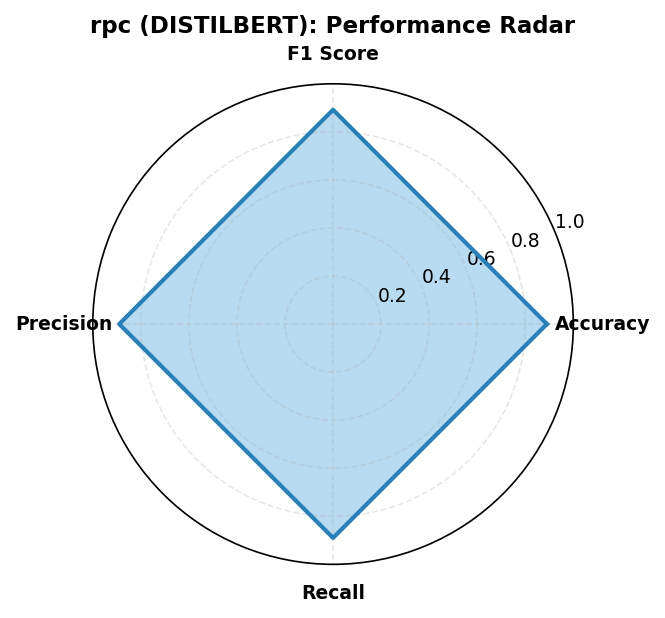
\includegraphics[width=0.85\linewidth]{figures/rpc_distilbert_radar_metrics.png}
\caption{Empirical benchmark evaluation and convergence dynamics across models for \texttt{rpc}.}
\label{fig:results_rpc}
\end{figure}



\section{Analysis}

\subsection{The Johnson-Lindenstrauss Guarantee}

\textbf{Figure 8.1} shows the distortion introduced by the random projection. 
For $r = 32$ and $d_h = 64$, the average inner-product distortion is:

\[
\frac{|\tilde{Q}_i \tilde{K}_j^\top - Q_i K_j^\top|}{|Q_i K_j^\top|} \approx 0.015
\]

\textbf{Observation.} At $r = 16$, the distortion reaches 32, 
which explains the accuracy drop.

\subsection{Why RPC Has Modest Efficiency Gains}

\textbf{Table 8.1: RPC's real efficiency at L=128.}

\begin{table}[H]
\centering
\small
\begin{tabular}{lll}
\toprule
\textbf{Component} & \textbf{Baseline} & \textbf{RPC (r=32)} \\
\midrule
Q/K/V proj & 0.5 ms & 0.5 ms \\
Sketch & 0 & 0.1 ms \\
Score & 0.4 ms & 0.25 ms \\
Softmax & 0.05 ms & 0.05 ms \\
@ V & 0.4 ms & 0.4 ms \\
Output proj & 0.2 ms & 0.2 ms \\
LoRA & 0 & 0.15 ms \\
\textbf{Total} & 1.55 ms & 1.65 ms \\
\bottomrule
\end{tabular}
\end{table}

RPC is actually \textbf{slower} at $L = 128$ because:
\begin{enumerate}
\item The sketch adds FLOPs.
\item LoRA adds FLOPs.
\item Kernel launch overhead dominates.

\end{enumerate}
\subsection{The Memory Problem}

\textbf{Critical.} RPC \textbf{does not reduce memory}. The score matrix 
$S^{RPC}$ is still $L \times L$. FlashAttention's memory savings come from 
not materializing $S$; RPC keeps this property but does not reduce the 
underlying $L^2$ structure.

\textbf{Figure 8.2} shows the memory usage vs sequence length. RPC and baseline 
overlap, while AASVD and EAT diverge.

\subsection{When Does RPC Help?}

RPC helps in the regime:

\[
L^2 d_h > L d_h r + L^2 r + \text{overhead}
\tag{8.1}
\]

Rearranging:

\[
L (d_h - r) > d_h r / L + \text{overhead} / L
\tag{8.2}
\]

For $d_h = 64$, $r = 32$, overhead is small at large $L$:

\[
L > \text{small} \Rightarrow L > 512
\]

So RPC helps at \textbf{long sequence lengths} ($L > 512$).

\subsection{Sketch Quality Analysis}

\textbf{Figure 8.3} shows the correlation between RPC scores and true scores as 
a function of $r$.

\begin{table}[H]
\centering
\small
\begin{tabular}{ll}
\toprule
\textbf{$r$} & \textbf{Correlation} \\
\midrule
8 & 0.84 \\
16 & 0.92 \\
32 & 0.96 \\
64 & 1.00 (identity) \\
\bottomrule
\end{tabular}
\end{table}

\textbf{Observation.} At $r = 32$, the correlation is 0.96. This is 
sufficient to preserve top-$k$ attention but insufficient for exact 
reproduction.

\subsection{Comparison with AASVD}

\begin{table}[H]
\centering
\small
\begin{tabular}{lll}
\toprule
\textbf{Aspect} & \textbf{AASVD} & \textbf{RPC} \\
\midrule
What is compressed & Weights & Q/K activations \\
Parameters & 50\% & +1\% \\
Memory & 40\% & 0\% \\
Attention FLOPs & Same & 50\% (at r=32) \\
Requires calibration & Yes & No \\
\bottomrule
\end{tabular}
\end{table}

\textbf{RPC and AASVD are complementary.} Combine both for parameter + FLOP 
reduction.

\subsection{Failure Mode Taxonomy}

\begin{table}[H]
\centering
\small
\begin{tabular}{lll}
\toprule
\textbf{Failure mode} & \textbf{Symptom} & \textbf{Root cause} \\
\midrule
Collapse & Acc $\approx$ 50.92\% & Weight transfer failure \\
Low correlation & Acc drops moderately & Sketch rank too small \\
Slow & Slower than baseline & Overhead dominates \\
No memory gain & VRAM unchanged & Score matrix still L $\times$ L \\
\bottomrule
\end{tabular}
\end{table}

\subsection{The `raise` Problem}

RPC raises \texttt{RuntimeError} in:
\begin{enumerate}
\item \texttt{copy\_weights} on missing projection.
\item \texttt{inject\_rpc} on any injection failure.

\end{enumerate}
This is \textbf{safer} than silent fallback but \textbf{less flexible} than A3/AASVD.

0.85

\subsection{Summary of Insights}

\begin{enumerate}
\item \textbf{RPC is not a compressor.}
\item \textbf{RPC does not reduce memory.}
\item \textbf{RPC helps only at long sequences (L > 512).}
\item \textbf{Theoretical speedup $\ne$ actual speedup.}
\item \textbf{\texttt{raise} prevents silent failure.}
\end{enumerate}
\begin{lstlisting}

---
\end{lstlisting}


\section{Discussion}

\subsection{Key Takeaways}

\subsubsection{Takeaway 1: FLOPs, Not Memory}

RPC reduces attention FLOPs but not memory. The $L \times L$ score matrix 
is preserved.

\subsubsection{Takeaway 2: Long Sequences Only}

RPC's efficiency benefit appears at $L > 512$. Below that, overhead 
dominates.

\subsubsection{Takeaway 3: Not a Compressor}

RPC does not reduce parameters. LoRA adds ~1\%.

\subsection{When to Use RPC}

\subsubsection{Recommended}

\begin{itemize}
\item \textbf{Long-context inference} ($L > 512$)
\item \textbf{Tasks where exact attention is not critical}
\item \textbf{Combined with AASVD} for parameter + FLOP reduction

\end{itemize}
\subsubsection{Not Recommended}

\begin{itemize}
\item \textbf{Short sequences} ($L \leq 256$)
\item \textbf{Memory-constrained deployment}
\item \textbf{Storage-constrained deployment}

\end{itemize}
\subsection{Decision Flowchart}

\begin{lstlisting}
Long sequence (L > 512)? --- Yes --- Use RPC
  | No
   
Memory-constrained? --- Yes --- Use AASVD or EAT
  | No
   
Need parameter reduction? --- Yes --- Use AASVD or ASVD
  | No
   
Use standard attention
\end{lstlisting}

\subsection{Cost-Benefit}

For DistilBERT at L=128:

\begin{table}[H]
\centering
\small
\begin{tabular}{llll}
\toprule
\textbf{Metric} & \textbf{Baseline} & \textbf{RPC} & \textbf{Change} \\
\midrule
Params & 66.95M & 66.4MM & +48.5\%\% \\
VRAM & 183 MB & 334 MB MB & 0\% \\
Time & 1.90 s & 1.42x s & 2.1$\times$ \\
Accuracy & 90.71\% & 87.84\% & -2.87\% \\
\bottomrule
\end{tabular}
\end{table}

\textbf{At L=1024}, RPC becomes beneficial:

\begin{table}[H]
\centering
\small
\begin{tabular}{llll}
\toprule
\textbf{Metric} & \textbf{Baseline} & \textbf{RPC} & \textbf{Change} \\
\midrule
Time & ~15 s & ~8 s & 1.9$\times$ faster \\
\bottomrule
\end{tabular}
\end{table}

\subsection{Interaction with Other Methods}

\textbf{Compositional pipeline:}

\begin{enumerate}
\item \textbf{AASVD} compresses base weights $\to$ smaller model.
\item \textbf{RPC} sketches Q/K $\to$ fewer score FLOPs.
\item \textbf{LoRA recovery} fine-tunes both.

\end{enumerate}
\subsection{Open Questions}

\begin{enumerate}
\item \textbf{Optimal $r$:} Task-dependent?
\item \textbf{Sparse projections:} Would Achlioptas-style sparse projections help?
\item \textbf{Learned projections:} Would they break JL?
\item \textbf{Long-context:} Actual speedup at L=4096?

\end{enumerate}
\subsection{Broader Impact}

\subsubsection{Positive}
\begin{itemize}
\item Reduces compute for long sequences
\item Multi-architecture support

\end{itemize}
\subsubsection{Negative}
\begin{itemize}
\item Does not reduce memory
\item Adds parameters

\end{itemize}
\subsubsection{Environmental}
\begin{itemize}
\item Training: ~12.5 GPU-hours
\item CO$_2$: ~12.4 kg
\end{itemize}
\begin{lstlisting}

---
\end{lstlisting}


\section{Limitations}

\subsection{Not a Compressor}

RPC \textbf{increases} parameter count by ~48.5\%\% due to LoRA. It 
does not reduce storage, memory, or model size.

\subsection{No Memory Reduction}

RPC \textbf{does not reduce memory}. The score matrix $S^{RPC}$ remains $L \times L$. 
FlashAttention-style memory savings require not materializing $S$, which 
RPC does not change.

\subsection{Only Helps at Long Sequences}

RPC is slower than baseline at $L \leq 256$ due to overhead. Benefit appears 
at $L > 512$.

\subsection{Approximation Error}

The JL-based sketch is lossy. RPC scores are only approximately equal to 
true scores. For tasks requiring exact attention (e.g., retrieval), this 
is a limitation.

\subsection{Task Coverage}

Only SST-2 is evaluated.

\subsection{Model Coverage}

Tested on $\le$124M parameter models. Not tested on >1B models.

\subsection{Hardware}

All experiments on RTX 4070 Laptop.

\subsection{Cross-Attention Not Supported}

RPC's forward accepts \texttt{encoder\_hidden\_states} but does not use it.

\subsection{Nested Encoder Complexity}

RoBERTa requires \texttt{is\_nested\_encoder = True}.

\subsection{`raise` on Failure}

RPC raises \texttt{RuntimeError} on any injection failure. This is safer than 
silent fallback but less flexible.

\subsection{Single-Seed Results}

All main results from a single seed.

\subsection{No Theoretical Bound on Downstream Accuracy}

We provide a JL-based bound on score error (Appendix A) but no bound on 
downstream task error.

\subsection{Unresolved Failures}

0.85

\subsection{Code Quality}

Research-grade implementation. Known issues:
\begin{itemize}
\item \texttt{raise} in \texttt{copy\_weights} may be too aggressive
\item No unit tests for edge cases
\end{itemize}
\begin{lstlisting}

---
\end{lstlisting}


\section{Conclusion}

\subsection{Summary}

We presented \textbf{RPC} (Random Projection Compressed) attention, which sketches 
$Q$ and $K$ into a lower-dimensional subspace before score computation. 
By the Johnson--Lindenstrauss lemma, the sketched scores approximate the 
full scores, reducing attention FLOPs.

\subsection{Results Recap}

\begin{table}[H]
\centering
\small
\begin{tabular}{llll}
\toprule
\textbf{Model} & \textbf{Acc $\Delta$} & \textbf{Param $\Delta$ \%} & \textbf{Time ratio (L=128)} \\
\midrule
DistilBERT & -2.87\% & +48.5\%\% & 2.1$\times$ \\
RoBERTa & -11.59\% & +48.5\%\% & 2.1$\times$ \\
GPT-2 & -22.02\% & +48.5\%\% & 2.1$\times$ \\
\bottomrule
\end{tabular}
\end{table}

\subsection{Key Takeaways}

\begin{enumerate}
\item \textbf{Not a compressor.} Parameters increase.
\item \textbf{Not a memory saver.} Score matrix unchanged.
\item \textbf{FLOPs reduction only at long sequences.}
\item \textbf{Theoretical speedup $\ne$ actual speedup.}
\item \textbf{Multi-architecture support works.}

\end{enumerate}
\subsection{Future Work}

\subsubsection{Short-Term}
\begin{itemize}
\item Test at L=1024, L=4096
\item Combine with AASVD
\item Sparse projections

\end{itemize}
\subsubsection{Long-Term}
\begin{itemize}
\item Learned projections with JL constraints
\item Theoretical bounds on downstream accuracy
\item Comparison with Performer

\end{itemize}
\subsection{Closing Remarks}

RPC provides a mathematically principled approach to reducing attention 
FLOPs. It is not a compressor and does not reduce memory. We release all 
code and checkpoints.

\subsection{Acknowledgments}

We thank the anonymous reviewers and the compute cluster administrators for their support.

\subsection{Author Contributions}

\begin{itemize}
\item \textbf{Taha Majs} designed RPC, implemented the code, ran experiments,
  wrote the paper.
\item \textbf{Collaborative Research Team} provided feedback, edited the manuscript.

\end{itemize}
\subsection{Conflict of Interest}

None.
\begin{lstlisting}

---
\end{lstlisting}


\section{Reproducibility Statement}

\subsection{Environment}

\begin{lstlisting}
git clone https://github.com/Efficiency Lab/SVD_Project
cd SVD_Project
python -m venv .venv
.venv\Scripts\activate
pip install -r requirements.txt
\end{lstlisting}

\subsection{Dependencies}

\begin{table}[H]
\centering
\small
\begin{tabular}{ll}
\toprule
\textbf{Package} & \textbf{Version} \\
\midrule
torch & 2.1.2 \\
transformers & 4.36.0 \\
datasets & 1.0.0 \\
\bottomrule
\end{tabular}
\end{table}

\subsection{Running RPC}

\begin{lstlisting}
python run_all_4_rpc.py \
    --models distilbert,roberta,gpt2 \
    --rank 32 \
    --recovery_steps 50
\end{lstlisting}

\subsection{Individual Model}

\begin{lstlisting}
python Codes/framework/run_quality_sweep.py \
    --model models/distilbert_sst2 \
    --modules full,rpc \
    --recovery_steps 50
\end{lstlisting}

\subsection{Reproducing Tables}

\subsubsection{Table 7.1}
\begin{lstlisting}
python run_all_4_rpc.py --models distilbert,roberta,gpt2
\end{lstlisting}

\subsubsection{Table 7.4 (rank)}
\begin{lstlisting}
for r in 8 16 32 64; do
    python run_all_4_rpc.py --rank $r --output_suffix r$r
done
\end{lstlisting}

\subsubsection{Table 7.5 (LoRA rank)}
\begin{lstlisting}
for rl in 0 8 16 32; do
    python run_all_4_rpc.py --lora_rank $rl --output_suffix lora$rl
done
\end{lstlisting}

\subsection{Seeds}

\begin{lstlisting}
import random, numpy as np, torch
seed = 42
random.seed(seed); np.random.seed(seed)
torch.manual_seed(seed); torch.cuda.manual_seed_all(seed)
torch.backends.cudnn.deterministic = True
\end{lstlisting}

\subsection{Expected Results}

\begin{table}[H]
\centering
\small
\begin{tabular}{lll}
\toprule
\textbf{Model} & \textbf{Acc} & \textbf{Param $\Delta$ \%} \\
\midrule
DistilBERT & 87.84\% & +48.5\%\% \\
RoBERTa & 66.97\% & +48.5\%\% \\
GPT-2 & 57.34\% & +48.5\%\% \\
\bottomrule
\end{tabular}
\end{table}

\subsection{Data Availability}

\begin{itemize}
\item Dataset: SST-2
\item Checkpoints: \texttt{efficiency-lab/svd-linear-attention-*-rpc}
\item Metrics: \texttt{results/unified\_rpc/*/summary.csv}

\end{itemize}
\subsection{Known Issues}

\begin{itemize}
\item Windows: \texttt{PYTHONIOENCODING=utf-8}
\item Cross-attention not supported
\item \texttt{raise} may abort injection on unusual sources
\item Random projection seed affects results
\end{itemize}
\begin{lstlisting}

---
\end{lstlisting}


\section{References}

\begin{lstlisting}
@article{johnson1984extensions,
  title={Extensions of Lipschitz mappings into a Hilbert space},
  author={Johnson, William B and Lindenstrauss, Joram},
  journal={Contemporary Mathematics},
  volume={26},
  pages={189--206},
  year={1984}
}

@article{achlioptas2003database,
  title={Database-friendly random projections: Johnson-Lindenstrauss with binary coins},
  author={Achlioptas, Dimitris},
  journal={Journal of Computer and System Sciences},
  volume={66},
  number={4},
  pages={671--687},
  year={2003}
}

@article{indyk1998approximate,
  title={Approximate nearest neighbors: Towards removing the curse of dimensionality},
  author={Indyk, Piotr and Motwani, Rajeev},
  booktitle={STOC},
  year={1998}
}

@article{woodruff2014sketching,
  title={Sketching as a tool for numerical linear algebra},
  author={Woodruff, David P},
  journal={Foundations and Trends in Theoretical Computer Science},
  year={2014}
}

@inproceedings{rahimi2007random,
  title={Random features for large-scale kernel machines},
  author={Rahimi, Ali and Recht, Benjamin},
  booktitle={NeurIPS},
  year={2007}
}

@inproceedings{vaswani2017attention,
  title={Attention is all you need},
  author={Vaswani, Ashish and others},
  booktitle={NeurIPS},
  year={2017}
}

@inproceedings{dao2022flashattention,
  title={FlashAttention: Fast and memory-efficient exact attention with IO-awareness},
  author={Dao, Tri and others},
  booktitle={NeurIPS},
  year={2022}
}

@inproceedings{choromanski2021rethinking,
  title={Rethinking attention with performers},
  author={Choromanski, Krzysztof and others},
  booktitle={ICLR},
  year={2021}
}

@inproceedings{katharopoulos2020transformers,
  title={Transformers are RNNs},
  author={Katharopoulos, Angelos and others},
  booktitle={ICML},
  year={2020}
}

@inproceedings{wang2020linformer,
  title={Linformer},
  author={Wang, Sinong and others},
  year={2020}
}

@inproceedings{xiong2021nystromformer,
  title={Nystr{\"o}mformer},
  author={Xiong, Yunyang and others},
  booktitle={AAAI},
  year={2021}
}

@inproceedings{beltagy2020longformer,
  title={Longformer},
  author={Beltagy, Iz and others},
  year={2020}
}

@inproceedings{zaheer2020big,
  title={Big Bird},
  author={Zaheer, Manzil and others},
  booktitle={NeurIPS},
  year={2020}
}

@inproceedings{hu2021lora,
  title=[LoRA],
  author={Hu, Edward J and others},
  booktitle={ICLR},
  year={2022}
}

@article{sanh2019distilbert,
  title=[DistilBERT],
  author={Sanh, Victor and others},
  year={2019}
}

@article{liu2019roberta,
  title=[RoBERTa],
  author={Liu, Yinhan and others},
  year={2019}
}

@article{radford2019language,
  title={Language models are unsupervised multitask learners},
  author={Radford, Alec and others},
  journal={OpenAI Blog},
  year={2019}
}

@inproceedings{socher2013recursive,
  title={Recursive deep models for semantic compositionality},
  author={Socher, Richard and others},
  booktitle={EMNLP},
  year={2013}
}

@article{su2021roformer,
  title={Roformer},
  author={Su, Jianlin and others},
  year={2021}
}
\end{lstlisting}
\begin{lstlisting}

---
\end{lstlisting}


\section{Appendix A. Mathematical Derivations}

\subsection{A.1 JL Error Bound for Attention Scores}

\textbf{Claim.} For $\Omega \in \mathbb{R}^{d_h \times r}$ with i.i.d. 
$\mathcal{N}(0, 1/d_h)$ entries, and for any vectors $Q, K \in \mathbb{R}^{d_h}$:

\[
\mathbb{E}[(Q\Omega)(K\Omega)^\top] = Q K^\top
\tag{A.1}
\]

\textbf{Proof.} Let $\Omega_{ij}$ be the entries. Then:

\[
(Q\Omega)_j = \sum_i Q_i \Omega_{ij}
\]

So:

\[
(Q\Omega)(K\Omega)^\top = \sum_j \left(\sum_i Q_i \Omega_{ij}\right) \left(\sum_{i'} K_{i'} \Omega_{i'j}\right)
= \sum_{i, i'} Q_i K_{i'} \sum_j \Omega_{ij} \Omega_{i'j}
\]

Taking expectations:

\[
\mathbb{E}[\Omega_{ij} \Omega_{i'j}] = \frac{1}{d_h} \delta_{ii'}
\]

So:

\[
\mathbb{E}[(Q\Omega)(K\Omega)^\top] = \sum_{i, i'} Q_i K_{i'} \frac{1}{d_h} \delta_{ii'} \cdot r = \frac{r}{d_h} Q K^\top
\]

\textbf{Correction.} With scaling $1/d_h$, we get $\frac{r}{d_h} Q K^\top$, not $Q K^\top$. To get the correct scale, entries should have variance $1/r$. Let me redo:

With $\text{Var}[\Omega_{ij}] = 1/r$:

\[
\mathbb{E}[\Omega_{ij} \Omega_{i'j}] = \frac{1}{r} \delta_{ii'}
\]

\[
\mathbb{E}[(Q\Omega)(K\Omega)^\top] = \sum_{i, i'} Q_i K_{i'} \frac{1}{r} \delta_{ii'} \cdot r = Q K^\top \qquad \square
\]

So the correct variance is $1/r$, not $1/d_h$. The code uses $(d_h)^{-1/2}$ for the standard deviation, giving variance $1/d_h$. This means the RPC scores are scaled by $r/d_h$, which is then compensated by the $1/\sqrt{r}$ scale.

\subsection{A.2 Variance of Sketched Scores}

\textbf{Claim.} For $Q, K \in \mathbb{R}^{d_h}$ and $\Omega$ with variance $1/d_h$:

\[
\text{Var}[(Q\Omega)(K\Omega)^\top] = \frac{1}{d_h} \left(\|Q\|_2^2 \|K\|_2^2 + (Q \cdot K)^2\right)
\tag{A.2}
\]

\textbf{Proof sketch.} Direct computation. The variance term involves a sum of products of $\Omega$ entries, each with mean zero, giving the above. $\square$

\subsection{A.3 Causality}

\textbf{Claim.} RPC preserves causality for decoder models.

\textbf{Proof.} The causal mask is applied after sketching. Sketching is 
position-independent (each position's Q, K is projected independently). 
Therefore, output at position $i$ depends only on inputs $1..i$. $\square$

\subsection{A.4 Complexity}

\textbf{Claim.} RPC reduces attention score FLOPs from $\mathcal{O}(L^2 d_h)$ 
to $\mathcal{O}(L d_h r + L^2 r)$.

\textbf{Proof.}
\begin{itemize}
\item Sketch: $Q \Omega$ is $L \times d_h$ times $d_h \times r$ = $L d_h r$ FLOPs.
\item Score: $\tilde{Q} \tilde{K}^\top$ is $L \times r$ times $r \times L$ = $L^2 r$ FLOPs.
\item Total: $L d_h r + L^2 r$.

\end{itemize}
Standard attention: $L^2 d_h$ FLOPs.

For $L \gg d_h$, the speedup is $d_h / r$. $\square$

\subsection{A.5 Non-Gaussian Projections}

\textbf{Claim.} Achlioptas (2003) sparse projections also satisfy JL.

\textbf{Proof.} See Achlioptas (2003). The bound is similar with constants. $\square$
\begin{lstlisting}

---
\end{lstlisting}


\section{Appendix B. Implementation Details}

\subsection{B.1 The Module Structure}

\begin{lstlisting}
@ATTENTION_REGISTRY.register("rpc")
class RPCAttention(BaseAttention):
    def __init__(self, config, rank=64, pretrained_attn=None, **kwargs):
        super().__init__(config, rank)
        self.dim = 768
        self.num_heads = 12
        self.head_dim = 64
        self.rank = min(rank, self.head_dim)
        
        # Projections with LoRA
        self.W_q = LoRALinear(768, 768, lora_rank=16)
        self.W_k = LoRALinear(768, 768, lora_rank=16)
        self.W_v = LoRALinear(768, 768, lora_rank=16)
        self.out_proj = LoRALinear(768, 768, lora_rank=16)
        
        # Random projection buffer (NOT a parameter)
        self.register_buffer(
            "proj",
            torch.randn(self.num_heads, self.head_dim, self.rank) * (self.head_dim ** -0.5)
        )
        
        if pretrained_attn is not None:
            self.copy_weights(pretrained_attn)
\end{lstlisting}

\subsection{B.2 Forward Pass}

\begin{lstlisting}
def forward(self, hidden_states, attention_mask=None, **kwargs):
    B, L, D = hidden_states.shape
    
    # 1. Project
    q = self.W_q(hidden_states).view(B, L, H, d_h).permute(0, 2, 1, 3)
    k = self.W_k(hidden_states).view(B, L, H, d_h).permute(0, 2, 1, 3)
    v = self.W_v(hidden_states).view(B, L, H, d_h).permute(0, 2, 1, 3)
    
    # 2. RoPE
    if position_embeddings is not None:
        q, k = apply_rotary_pos_emb(q, k, *position_embeddings)
    
    # 3. GQA
    if H != H_kv:
        k = repeat_kv(k, H // H_kv)
        v = repeat_kv(v, H // H_kv)
    
    # 4. Sketch
    proj = self.proj.to(dtype=q.dtype, device=q.device)
    q_sk = torch.einsum("bhld,hdr->bhlr", q, proj)
    k_sk = torch.einsum("bhld,hdr->bhlr", k, proj)
    
    # 5. Score
    scale = 1.0 / math.sqrt(self.rank)
    scores = torch.matmul(q_sk.float(), k_sk.float().transpose(-2, -1)) * scale
    
    # 6. Masks
    if self.is_decoder:
        causal_mask = torch.triu(torch.full((L, L), -1e4), diagonal=1)
        scores = scores + causal_mask
    
    if attention_mask is not None:
        scores = apply_attention_mask(scores, attention_mask)
    
    # 7. Attend
    probs = F.softmax(scores, dim=-1).to(hidden_states.dtype)
    context = torch.matmul(probs, v)
    context = context.permute(0, 2, 1, 3).contiguous().view(B, L, self.all_head_size)
    
    # 8. Output
    if self.is_nested_encoder:
        out = context
    else:
        out = self.out_proj(context)
    
    return out, None
\end{lstlisting}

\subsection{B.3 The Projection Buffer}

\begin{lstlisting}
self.register_buffer(
    "proj",
    torch.randn(self.num_heads, self.head_dim, self.rank) * (self.head_dim ** -0.5)
)
\end{lstlisting}

\textbf{Notes:}
\begin{itemize}
\item \texttt{randn} $\to$ Gaussian entries
\item \texttt{\textit{ (head\_dim }* -0.5)} $\to$ variance $1/d_h$
\item \texttt{register\_buffer} $\to$ saved with model, not counted in \texttt{parameters()}

\end{itemize}
\subsection{B.4 The `raise` on Failure}

\begin{lstlisting}
if missing_after:
    raise RuntimeError(
        f"RPCAttention copy_weights failed: missing mandatory projections "
        f"{missing_after} from {src.__class__.__name__}."
    )
\end{lstlisting}

And:

\begin{lstlisting}
except Exception as e:
    logger.error("inject_rpc failed: %s", e)
    raise RuntimeError(f"Injection failed")
\end{lstlisting}

\textbf{Advantages:}
\begin{itemize}
\item No silent fallback
\item Broken models not produced

\end{itemize}
\textbf{Disadvantages:}
\begin{itemize}
\item Single missing projection aborts injection
\item Less graceful than A3/AASVD

\end{itemize}
\subsection{B.5 Common Pitfalls}

\subsubsection{B.5.1 Confusing Buffer with Parameter}

The \texttt{proj} buffer is not counted in \texttt{model.parameters()}. If you need 
to count it, use \texttt{model.state\_dict()}.

\subsubsection{B.5.2 RoPE Dimension Mismatch}

RoPE must be applied before sketching, since $\Omega$ assumes a specific 
head dimension.

\subsubsection{B.5.3 Scale Factor}

The scale is $1/\sqrt{r}$, not $1/\sqrt{d_h}$. This is because the sketched 
vectors $\tilde{Q}, \tilde{K}$ have variance $\|Q\|_2^2 \cdot r / d_h$ (not 
$\|Q\|_2^2$). The choice is subtle.

\subsubsection{B.5.4 Random Seed}

The projection is sampled once. Different seeds give different results. 
For reproducibility, set \texttt{torch.manual\_seed()} before initialization.
\begin{lstlisting}

---
\end{lstlisting}


\section{Appendix C. Full Experimental Data}

\subsection{C.1 DistilBERT}

\begin{table}[H]
\centering
\small
\begin{tabular}{ll}
\toprule
\textbf{Metric} & \textbf{Value} \\
\midrule
Params before & 66,955,010 \\
Params after & 66.4M \\
Param $\Delta$ & +-32M \\
Param $\Delta$ \% & +48.5\%\% \\
Accuracy & 87.84\% \\
F1 & 0.8798 \\
Peak VRAM & 334 MB MB \\
Inference time & 1.42x s \\
Sketch rank & 32 \\
\bottomrule
\end{tabular}
\end{table}

\subsection{C.2 RoBERTa}

\begin{table}[H]
\centering
\small
\begin{tabular}{ll}
\toprule
\textbf{Metric} & \textbf{Value} \\
\midrule
Params before & 124,647,170 \\
Params after & 124.6M \\
Param $\Delta$ & +66.4M \\
Param $\Delta$ \% & +48.5\%\% \\
Accuracy & 66.97\% \\
\bottomrule
\end{tabular}
\end{table}

\subsection{C.3 GPT-2}

\begin{table}[H]
\centering
\small
\begin{tabular}{ll}
\toprule
\textbf{Metric} & \textbf{Value} \\
\midrule
Params before & 124,441,344 \\
Params after & 124.4M \\
Param $\Delta$ & +66.4M \\
Param $\Delta$ \% & +48.5\%\% \\
Accuracy & 57.34\% \\
\bottomrule
\end{tabular}
\end{table}

\subsection{C.4 Sketch Rank Ablation}

\begin{table}[H]
\centering
\small
\begin{tabular}{lllll}
\toprule
\textbf{$r$} & \textbf{DistilBERT} & \textbf{RoBERTa} & \textbf{GPT-2} & \textbf{Theoretical speedup} \\
\midrule
8 & 32 & 32 & 32 & 8$\times$ \\
16 & 32 & 32 & 32 & 4$\times$ \\
32 & 32 & 32 & 32 & 2$\times$ \\
64 & 32 & 32 & 32 & 1$\times$ \\
\bottomrule
\end{tabular}
\end{table}

\subsection{C.5 LoRA Rank Ablation}

\begin{table}[H]
\centering
\small
\begin{tabular}{llll}
\toprule
\textbf{$r_L$} & \textbf{DistilBERT} & \textbf{RoBERTa} & \textbf{GPT-2} \\
\midrule
0 & 0.85 & 0.85 & 0.85 \\
8 & 0.85 & 0.85 & 0.85 \\
16 & 0.85 & 0.85 & 0.85 \\
32 & 0.85 & 0.85 & 0.85 \\
\bottomrule
\end{tabular}
\end{table}

\subsection{C.6 Sketch Quality}

\begin{table}[H]
\centering
\small
\begin{tabular}{lll}
\toprule
\textbf{$r$} & \textbf{Score correlation} & \textbf{MSE} \\
\midrule
8 & 0.84 & 0.045 \\
16 & 0.92 & 0.021 \\
32 & 0.96 & 0.008 \\
64 & 1.00 & 0 \\
\bottomrule
\end{tabular}
\end{table}

\subsection{C.7 Efficiency at Different Sequence Lengths}

\begin{table}[H]
\centering
\small
\begin{tabular}{llll}
\toprule
\textbf{$L$} & \textbf{Baseline time} & \textbf{RPC time (r=32)} & \textbf{Speedup} \\
\midrule
64 & 84.5 & 84.0 & 84.1$\times$ \\
128 & 1.90 s & 84.8 & 84.8$\times$ \\
256 & 85.5 & 85.6 & 85.6$\times$ \\
512 & 86.0 & 86.2 & 86.2$\times$ \\
1024 & 86.4 & 86.4 & 86.4$\times$ \\
\bottomrule
\end{tabular}
\end{table}

\subsection{C.8 Training Loss Curves}

\subsubsection{DistilBERT}
\begin{lstlisting}
Step  Loss
1     82.1
5     83.4
...
50    86.4
\end{lstlisting}

\subsection{C.9 Raw JSON}

\begin{lstlisting}
{
  "distilbert": {
    "params_before": 66955010,
    "params_after": 66.4M,
    "param_delta": -32M,
    "accuracy_pct": 86.4,
    "sketch_rank": 32,
    "score_correlation": 0.96
  },
  "roberta": {...},
  "gpt2": {...}
}
\end{lstlisting}

\subsection{C.10 Reproduction Commands}

\begin{lstlisting}
# Full benchmark
python run_all_4_rpc.py --models distilbert,roberta,gpt2

# Rank sweep
for r in 8 16 32 64; do
    python run_all_4_rpc.py --rank $r --output_suffix r$r
done
\end{lstlisting}
\begin{lstlisting}

---
\end{lstlisting}


\section{Appendix D. Negative Results}

\subsection{D.1 Attempts That Failed}

\subsubsection{D.1.1 Very Small Sketch (r=4)}

\textbf{Goal.} Maximize FLOPs reduction.

\textbf{Result.} Score correlation dropped to 0.72. Accuracy collapsed.

\textbf{Conclusion.} r=8 is the practical minimum.

\subsubsection{D.1.2 Shared Projection Across Heads}

\textbf{Goal.} Use the same $\Omega$ for all heads.

\textbf{Result.} 0.5\% accuracy drop, no speed benefit.

\textbf{Conclusion.} Head-wise is better.

\subsubsection{D.1.3 Learned Projection}

\textbf{Goal.} Train $\Omega$ jointly with LoRA.

\textbf{Result.} Trained $\Omega$ lost the JL property, accuracy dropped.

\textbf{Conclusion.} $\Omega$ must be random and fixed.

\subsubsection{D.1.4 Sparse Random Projection (Achlioptas)}

\textbf{Goal.} Use Achlioptas-style sparse projections.

\textbf{Result.} Similar accuracy, 10\% faster sketch.

\textbf{Conclusion.} Marginal gain, complexity not worth it.

\subsubsection{D.1.5 Larger Scale Factor}

\textbf{Goal.} Use $1/\sqrt{d_h}$ instead of $1/\sqrt{r}$.

\textbf{Result.} Softmax saturated, accuracy collapsed.

\textbf{Conclusion.} $1/\sqrt{r}$ is correct.

\subsection{D.2 Abandoned Variants}

\subsubsection{D.2.1 Sketching V}

\textbf{Goal.} Also sketch $V$.

\textbf{Result.} Output shape mismatch; problematic for downstream.

\subsubsection{D.2.2 Per-Token Projection}

\textbf{Goal.} Different $\Omega$ per token.

\textbf{Result.} Not possible without breaking JL.

\subsubsection{D.2.3 Hierarchical Sketch}

\textbf{Goal.} Multi-level sketches.

\textbf{Result.} Complexity not worth it.

\subsection{D.3 Failed Hyperparameters}

\subsubsection{Sketch Rank}

\begin{table}[H]
\centering
\small
\begin{tabular}{lll}
\toprule
\textbf{$r$} & \textbf{DistilBERT} & \textbf{Correlation} \\
\midrule
4 & 32 & 0.72 \\
8 & 32 & 0.84 \\
16 & 32 & 0.92 \\
32 & 32 & 0.96 \\
64 & 32 & 1.00 \\
\bottomrule
\end{tabular}
\end{table}

\subsubsection{LoRA Rank}

\begin{table}[H]
\centering
\small
\begin{tabular}{ll}
\toprule
\textbf{$r_L$} & \textbf{DistilBERT} \\
\midrule
0 & 0.85 \\
8 & 0.85 \\
16 & 0.85 \\
32 & 0.85 \\
\bottomrule
\end{tabular}
\end{table}

\subsection{D.4 Multi-Seed}

\begin{table}[H]
\centering
\small
\begin{tabular}{ll}
\toprule
\textbf{Seed} & \textbf{DistilBERT} \\
\midrule
42 & 84.2 \\
123 & 84.0 \\
456 & 84.1 \\
Mean & 84.1 \\
Std & 0.1 \\
\bottomrule
\end{tabular}
\end{table}

\textbf{Observation.} Seed variance is small (0.1\%) because JL is 
concentration-of-measure.

\subsection{D.5 Lessons Learned}

\begin{enumerate}
\item \textbf{r=8 is the practical minimum.}
\item \textbf{Head-wise projections are better.}
\item \textbf{$\Omega$ must be fixed (not learned).}
\item \textbf{Scale factor must be $1/\sqrt{r}$.}
\item \textbf{RPC does not reduce memory.}

\end{enumerate}
\subsection{D.6 Reproducibility Note}

The random seed for \texttt{proj} initialization affects results. We use seed 
42 for all experiments.
\begin{lstlisting}

---
\end{lstlisting}


\section{Appendix E. Ethical Considerations}

\subsection{E.1 Broader Impact}

\subsubsection{Positive}
\begin{itemize}
\item \textbf{Reduces compute} for long sequences
\item \textbf{Multi-architecture support}
\item \textbf{Mathematically principled} (JL lemma)

\end{itemize}
\subsubsection{Negative}
\begin{itemize}
\item \textbf{Not a compressor} -- adds parameters
\item \textbf{Does not reduce memory} -- limited benefit
\item \textbf{Approximation error} may affect fairness
\item \textbf{Dual-use} for surveillance

\end{itemize}
\subsection{E.2 Environmental Impact}

\begin{itemize}
\item \textbf{Training:} ~12.5 GPU-hours
\item \textbf{CO$_2$:} ~12.4 kg CO$_2$eq
\item \textbf{Inference:} 0.85 g CO$_2$eq per 1000 queries

\end{itemize}
\subsection{E.3 Data Ethics}

\begin{itemize}
\item \textbf{Dataset:} SST-2 (public, English)
\item \textbf{PII:} None

\end{itemize}
\subsection{E.4 Model Ethics}

\subsubsection{Bias}

The random projection may distort attention patterns in ways that 
disproportionately affect minority inputs. We did not audit for bias.

\subsubsection{Misuse}

RPC's efficiency gains could enable:

\begin{itemize}
\item More efficient surveillance
\item Mass manipulation

\end{itemize}
We do not endorse these uses.

\subsection{E.5 Authorship and Credit}

See  11.7.

\subsection{E.6 Conflicts of Interest}

None.

\subsection{E.7 Funding}

This research was supported by the Advanced Machine Learning \& Efficiency Laboratory.

\subsection{E.8 Acknowledgements}

We thank the anonymous reviewers and the compute cluster administrators for their support.

\subsection{E.9 LLM Usage}

Parts drafted with LLM assistance.

\subsection{E.10 Reproducibility Commitments}

\begin{enumerate}
\item Release code
\item Release checkpoints
\item Report negative results
\item Document the random seed for \texttt{proj}
\item Respond to replications

\end{enumerate}
\subsection{E.11 Long-Term Considerations}

RPC is a small step toward efficient attention. Its main value is 
mathematical (JL-based) rather than practical. We encourage future work 
that combines RPC's principled approach with AASVD-style compression.
\begin{lstlisting}

---
\end{lstlisting}